\documentclass[]{beamer}

\usepackage[ngerman]{babel}
\usepackage[utf8]{inputenc}
\usepackage{amsmath,amsfonts,amssymb}

\usetheme{Frankfurt}
\usecolortheme{beaver}
\usefonttheme{default}
\useinnertheme{rounded}
\useoutertheme{default}
\usepackage{graphicx}

\title{How NAO learns to kick the ball ...}
\author{Jannick, André, Daniel, Florian}
\date{11.07.2012}
\titlegraphic{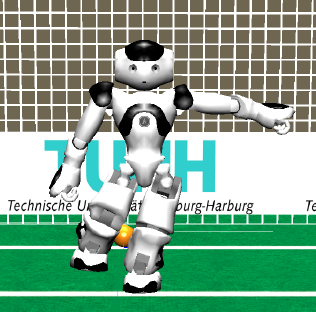
\includegraphics[scale=0.45]{nao}}

\begin{document}

%% frame 1
\begin{frame}
	\titlepage
\end{frame}
%% frame 1

\section*{Agenda}
%% frame 2
\begin{frame}
	\frametitle{Agenda}
  	\tableofcontents
\end{frame}
%% frame 2

\section{Einleitung}
%% frame 3
\begin{frame}
	\frametitle{Ziel des Seminars}
	
\end{frame}
%% frame 3

\section{Arbeitsschritte}
%% frame 4
\begin{frame}
	\frametitle{Arbeitsschritte}
	
\end{frame}
%% frame 4

\subsection{Phase 1}
%% frame 5
\begin{frame}
	\frametitle{Phase 1}
	
\end{frame}
%% frame 5

\subsection{Phase 2}
%% frame 6
\begin{frame}
	\frametitle{Phase 2}
	
\end{frame}
%% frame 6

\subsection{Phase 3}
%% frame 7
\begin{frame}
	\frametitle{Phase 3}
	
\end{frame}
%% frame 7	

\section{Ergebnis und Ausblick}
%% frame 8
\begin{frame}
	\frametitle{Ergebnis und Ausblick}
	
\end{frame}
%% frame 8

\section{Präsentation}	
%% frame 9
\begin{frame}
	\frametitle{Präsentation}
	
\end{frame}
%% frame 9
	
\end{document}